\subsection{Twelve high-input partitions: ten-minute evaluation}\label{sec:twelve-partition-updated}
The twelve-partition comparison used 700 aggregate messages/s over 60 partitions, with 80\% of traffic directed to twelve partitions initially owned by Consumer 2. Eight trials compared retaining the same three-consumer assignment, redistribution within three, scaling to six with targeted redistribution, and scaling to six with Kafka's normal cooperative rebalance. Each condition was run twice, reversing condition order in the second repetition. Starting ownership and the original consumers' pod identities, nodes and resource declarations were checked before traffic.

Every trial admitted 420,000 evaluation messages. Keeping the initial assignment left 34.64--34.83\% unfinished at cutoff; all interventions completed the cohort. Redistribution within three produced p99 latency of 80.10--84.16 seconds, compared with 100.81--107.24 seconds for targeted scaling and 71.41--72.46 seconds for normal Kafka scaling. The one-second cohort deadline-miss rates reveal a different aspect of the latency distribution: 30.50--31.84\% for redistribution, 26.26--27.33\% for targeted scaling and 21.05--25.83\% for normal scaling, versus 83.32--83.36\% without intervention. Thus a higher p99 does not imply more misses at every deadline.

The resource measurements show the trade-off. Redistribution used approximately 1,035--1,038 observed consumer CPU core-seconds over evaluation plus drain; targeted scaling used 1,310--1,327 and normal scaling 1,452--1,459. Requested CPU was 72 core-minutes for redistribution and approximately 137 for either six-consumer response. Actual RSS integrals were 2.53--2.65, 3.95--4.15 and 3.66--3.69 GiB-minutes respectively. These values concern consumer processes and resource declarations, not total infrastructure cost. The first unchanged baseline lacks almost all local request history and cannot support a full-window request-cost comparison; its message outcomes and recovered historical process measurements remain usable within their stated coverage.

Targeted scaling confirmed recovery sooner than redistribution within three (169.0--184.9 versus 305.2--328.9 seconds after the action decision), despite its higher whole-cohort p99. Recovery requires processing backlog at most 100 offsets for thirty consecutive valid seconds while input continues. Normal scaling's recovery varied from 143.0 to 259.0 seconds. Explicit ownership changes use a global release/acquire/resume barrier; their 14.40--14.54-second and 19.05--19.50-second processing pauses are distinguished from complete action duration. Normal cooperative scaling had much shorter global gaps, which does not imply every partition processed continuously.

Persistent hotspots were present before intervention. In the redistribution and targeted-scaling runs, none remained at any defined snapshot in the final two evaluation minutes. The diagnostic figure also shows that relative skew may rise during successful backlog clearance: the maximum and mean absolute partition lags are then small. Persistence and skew are useful descriptions of concentration, but neither alone establishes overload.

Processing-start mean latency ranged from 7.552 to 160.117 seconds across this block; it remains separate from completion latency. Every trial achieved 700 acknowledged evaluation messages/s. No duplicate completion attempts were detected, so completed-attempt and distinct-completion throughput coincide in these trials. Mean application work is reported below; it excludes evidence-writing and offset-commit overhead.
Observed per-process CPU coverage over evaluation plus drain ranged from 87.50\% to 99.72\%. Coverage uses the complete observation window, including time before additional consumers started; a lower value for a newly started consumer is not automatically a monitoring failure. The integral includes only observed valid process intervals.
\begin{table}[!htbp]
\centering\small
\setlength{\tabcolsep}{3pt}
\renewcommand{\arraystretch}{1.12}
\begin{tabular}{@{}lrrrrr@{}}
\toprule
Response & Run & \shortstack{p99\\(s)} & \shortstack{Unfinished\\(\%)} & \shortstack{Misses $>1$ s\\(\%)} & \shortstack{Useful throughput\\(msg/s)}\\
\midrule
Keep 3 & 1 & 366.64 & 34.641 & 83.32 & 423.23\\
Keep 3 & 2 & 362.79 & 34.828 & 83.36 & 422.62\\
Redistribute 3 & 1 & 80.10 & 0.000 & 30.50 & 727.71\\
Redistribute 3 & 2 & 84.16 & 0.000 & 31.84 & 729.53\\
Targeted scale 6 & 1 & 100.81 & 0.000 & 26.26 & 727.75\\
Targeted scale 6 & 2 & 107.24 & 0.000 & 27.33 & 729.31\\
Kafka scale 6 & 1 & 71.41 & 0.000 & 25.83 & 727.65\\
Kafka scale 6 & 2 & 72.46 & 0.000 & 21.05 & 728.48\\
\bottomrule
\end{tabular}
\caption{Whole evaluation-born cohort through the fixed drain cutoff. Deadline misses include overdue unfinished messages. Useful throughput counts distinct completions during evaluation, including warm-up records completed then; it can exceed the input rate while queued work is cleared.}
\label{tab:twelve-partition-outcomes}
\end{table}
\begin{table}[!htbp]
\centering\small
\setlength{\tabcolsep}{3pt}
\renewcommand{\arraystretch}{1.12}
\begin{tabular}{@{}lrrrrr@{}}
\toprule
Response & Run & \shortstack{Actual CPU\\(core-s)} & \shortstack{Actual RSS\\(GiB-min)} & \shortstack{Requested CPU\\(core-min)} & \shortstack{Requested memory\\(GiB-min)}\\
\midrule
Keep 3 & 1 & 892.9 & 3.24 & --- & ---\\
Keep 3 & 2 & 889.7 & 3.24 & 72.00 & 36.00\\
Redistribute 3 & 1 & 1,035.3 & 2.53 & 72.00 & 36.00\\
Redistribute 3 & 2 & 1,037.9 & 2.65 & 72.00 & 36.00\\
Targeted scale 6 & 1 & 1,310.5 & 4.15 & 136.86 & 68.43\\
Targeted scale 6 & 2 & 1,327.5 & 3.95 & 136.80 & 68.40\\
Kafka scale 6 & 1 & 1,451.5 & 3.66 & 137.15 & 68.58\\
Kafka scale 6 & 2 & 1,459.0 & 3.69 & 137.15 & 68.57\\
\bottomrule
\end{tabular}
\caption{Consumer resources over evaluation plus drain. Actual values integrate observed process CPU and RSS intervals and sum them across consumers. Requested values integrate Kubernetes resource declarations; neither is monetary or whole-cluster cost. A dash denotes unavailable full-window request coverage, not zero cost.}
\label{tab:twelve-partition-resources}
\end{table}
\begin{table}[!htbp]
\centering\small
\setlength{\tabcolsep}{3pt}
\renewcommand{\arraystretch}{1.12}
\begin{tabular}{@{}lrrrrrr@{}}
\toprule
Response & Run & \shortstack{Mean total\\lag} & \shortstack{Peak total\\lag} & \shortstack{Lag coverage\\(\%)} & \shortstack{Peak partition\\lag} & Mean skew\\
\midrule
Keep 3 & 1 & 98,929 & 180,743 & 99.7 & 14,752 & 4.90\\
Keep 3 & 2 & 100,033 & 182,438 & 99.7 & 14,794 & 4.90\\
Redistribute 3 & 1 & 7,837 & 46,048 & 96.3 & 5,536 & 9.92\\
Redistribute 3 & 2 & 8,664 & 47,675 & 96.3 & 5,883 & 10.30\\
Targeted scale 6 & 1 & 8,470 & 55,923 & 95.3 & 5,216 & 9.05\\
Targeted scale 6 & 2 & 9,520 & 60,387 & 95.3 & 5,544 & 9.31\\
Kafka scale 6 & 1 & 6,688 & 38,516 & 98.0 & 4,332 & 10.34\\
Kafka scale 6 & 2 & 5,702 & 40,065 & 98.0 & 4,510 & 8.91\\
\bottomrule
\end{tabular}
\caption{Lag diagnostics during evaluation only, in offsets except skew and coverage. Means use trapezoidal area divided by covered time; peaks are sampled maxima. The time mean of the skew ratio is not the ratio of time-averaged maximum and mean lag. Invalid samples and ownership changes are not bridged.}
\label{tab:twelve-partition-diagnostics}
\end{table}
\begin{table}[!htbp]
\centering\small
\setlength{\tabcolsep}{3pt}
\renewcommand{\arraystretch}{1.12}
\begin{tabular}{@{}lrrrrrr@{}}
\toprule
Response & Run & Mean (s) & p50 (s) & p95 (s) & \shortstack{Mean work\\(ms)} & \shortstack{Observed misses\\$>1$ s (\%)}\\
\midrule
Keep 3 & 1 & 158.994 & 161.677 & 341.123 & 2.613 & 72.41\\
Keep 3 & 2 & 160.120 & 164.185 & 344.752 & 2.614 & 72.45\\
Redistribute 3 & 1 & 11.585 & 0.099 & 62.417 & 1.956 & 33.16\\
Redistribute 3 & 2 & 12.676 & 0.100 & 65.276 & 1.943 & 34.61\\
Targeted scale 6 & 1 & 13.813 & 0.124 & 81.024 & 2.451 & 29.08\\
Targeted scale 6 & 2 & 15.245 & 0.125 & 87.387 & 2.457 & 30.27\\
Kafka scale 6 & 1 & 9.140 & 0.120 & 57.805 & 2.764 & 28.66\\
Kafka scale 6 & 2 & 7.555 & 0.120 & 57.333 & 2.773 & 24.15\\
\bottomrule
\end{tabular}
\caption{Supplementary latency diagnostics. Mean, p50 and p95 use completed evaluation-born messages. Mean work is the local monotonic application-processing duration. Observed violations use completion attempts occurring during evaluation and have a different denominator from the primary admitted-cohort deadline rate.}
\label{tab:twelve-partition-latency-details}
\end{table}
\begin{table}[!htbp]
\centering\small
\setlength{\tabcolsep}{3pt}
\renewcommand{\arraystretch}{1.12}
\begin{tabular}{@{}lrrrrrr@{}}
\toprule
Response & Run & \shortstack{Decision to\\active (s)} & \shortstack{Global gap\\(s)} & \shortstack{Extra pending\\during pause} & \shortstack{Net pending\\during transfer} & \shortstack{Recovery\\(s)}\\
\midrule
Keep 3 & 1 & --- & N/A & N/A & N/A & N/A\\
Keep 3 & 2 & --- & N/A & N/A & N/A & N/A\\
Redistribute 3 & 1 & 25.73 & 14.544 & 10,181 & 6,808 & 305.2\\
Redistribute 3 & 2 & 26.01 & 14.400 & 10,081 & 6,581 & 328.9\\
Targeted scale 6 & 1 & 72.81 & 19.498 & 13,648 & 2,082 & 169.0\\
Targeted scale 6 & 2 & 77.18 & 19.049 & 13,350 & 548 & 184.9\\
Kafka scale 6 & 1 & 31.01 & 0.092 & N/A & -6,777 & 259.0\\
Kafka scale 6 & 2 & 33.01 & 0.202 & N/A & -9,823 & 143.0\\
\bottomrule
\end{tabular}
\caption{Intervention costs. For targeted actions, transfer is release request to verified active ownership; for native scaling it is decision to stable-six-owner confirmation. The latter also defines native decision-to-active. Recovery is confirmation after the actual decision. Global gap measures the longest interval without any consumer processing, not a per-partition downtime. Negative net pending change means processing reduced outstanding work during the measured transition. Dashes denote unavailable or inapplicable values.}
\label{tab:twelve-partition-intervention-cost}
\end{table}
\begin{table}[!htbp]
\centering\small
\setlength{\tabcolsep}{3pt}
\renewcommand{\arraystretch}{1.12}
\begin{tabular}{@{}lrrrrrrr@{}}
\toprule
Response & Run & C0 & C1 & C2 & C3 & C4 & C5\\
\midrule
Keep 3 & 1 & 0 & 0 & 12 & --- & --- & ---\\
Keep 3 & 2 & 0 & 0 & 12 & --- & --- & ---\\
Redistribute 3 & 1 & 4 & 4 & 4 & --- & --- & ---\\
Redistribute 3 & 2 & 4 & 4 & 4 & --- & --- & ---\\
Targeted scale 6 & 1 & 2 & 2 & 2 & 2 & 2 & 2\\
Targeted scale 6 & 2 & 2 & 2 & 2 & 2 & 2 & 2\\
Kafka scale 6 & 1 & 0 & 0 & 2 & 4 & 2 & 4\\
Kafka scale 6 & 2 & 0 & 0 & 2 & 4 & 3 & 3\\
\bottomrule
\end{tabular}
\caption{Final observed numbers of configured high-input partitions per consumer. These are traffic targets, not persistent-hot detector counts. All high-input partitions initially belonged to Consumer 2. A dash means no observed partition ownership.}
\label{tab:twelve-partition-ownership}
\end{table}
\begin{table}[!htbp]
\centering\small
\setlength{\tabcolsep}{3pt}
\renewcommand{\arraystretch}{1.12}
\begin{tabular}{@{}lrrrrr@{}}
\toprule
Response & Run & Reference event & C3 (s) & C4 (s) & C5 (s)\\
\midrule
Targeted scale 6 & 1 & Replica request & 63.37 & 63.41 & 63.37\\
Targeted scale 6 & 2 & Replica request & 67.20 & 67.12 & 67.23\\
Kafka scale 6 & 1 & Action decision & 9.22 & 16.43 & 14.35\\
Kafka scale 6 & 2 & Action decision & 9.42 & 18.66 & 9.54\\
\bottomrule
\end{tabular}
\caption{Activation delay to the first valid completion on each added consumer. Targeted scaling uses the recorded replica-request event; native scaling uses the action decision because an equivalent replica-request timestamp was not separately recorded. These are not whole-action completion times or pure rebalance delays.}
\label{tab:twelve-partition-activation-delay}
\end{table}
\clearpage
\begin{figure}[p]
\centering
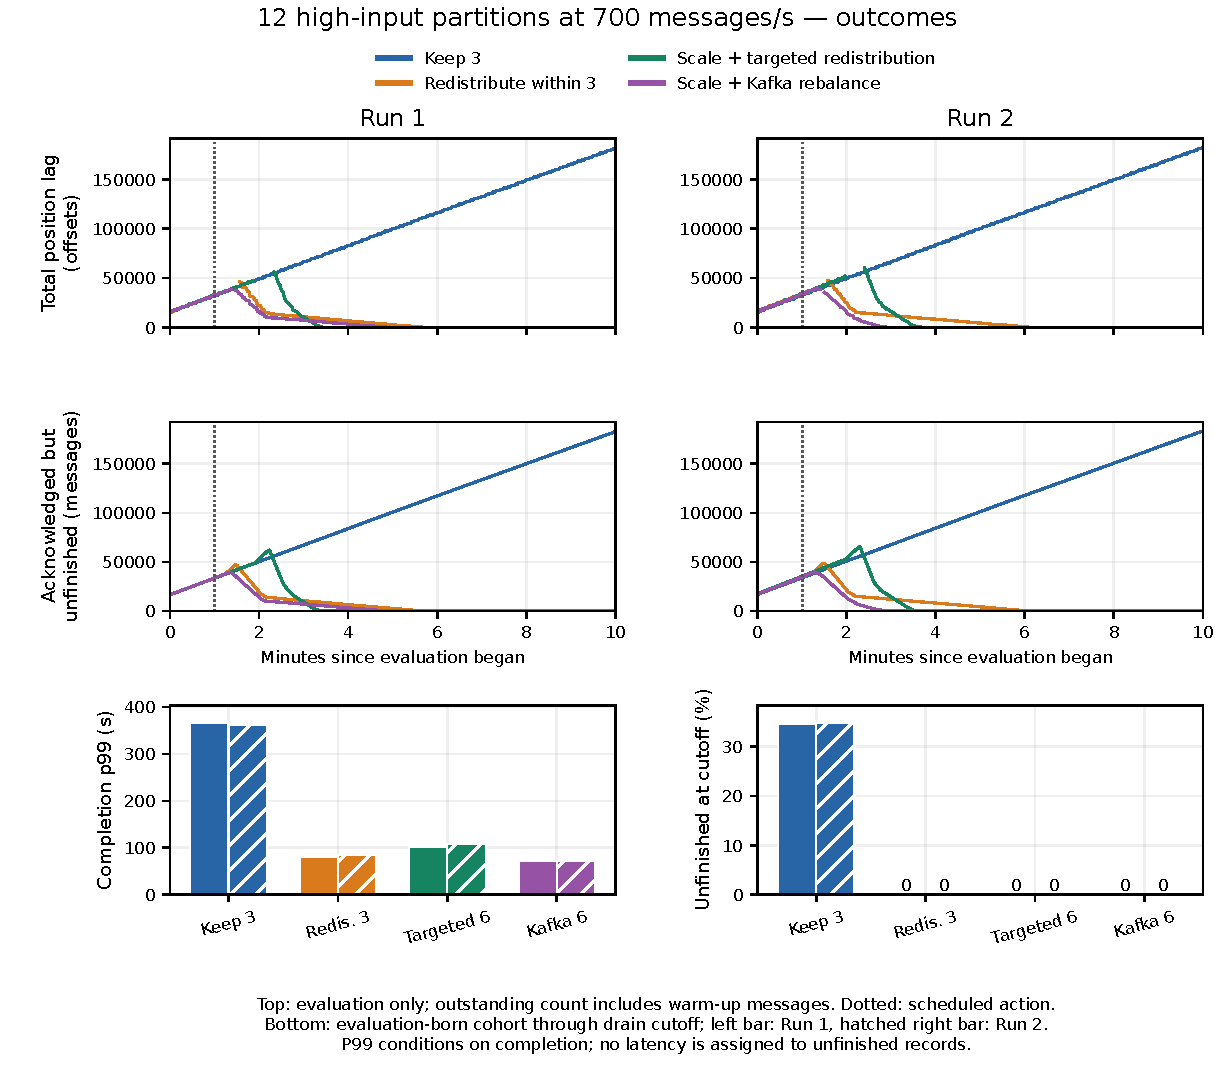
\includegraphics[width=\linewidth,height=.79\textheight,keepaspectratio]{figures/twelve-partition-compact-outcomes.pdf}
\caption{Compact outcome comparison: total consumer-position lag and exact acknowledged-but-unfinished work during evaluation, followed by whole-cohort p99 and unfinished percentage at the drain cutoff. Warm-up work is included in the time-series counts but excluded from the outcome cohort.}
\label{fig:twelve-partition-compact-outcomes}
\end{figure}
\clearpage
\begin{figure}[p]
\centering
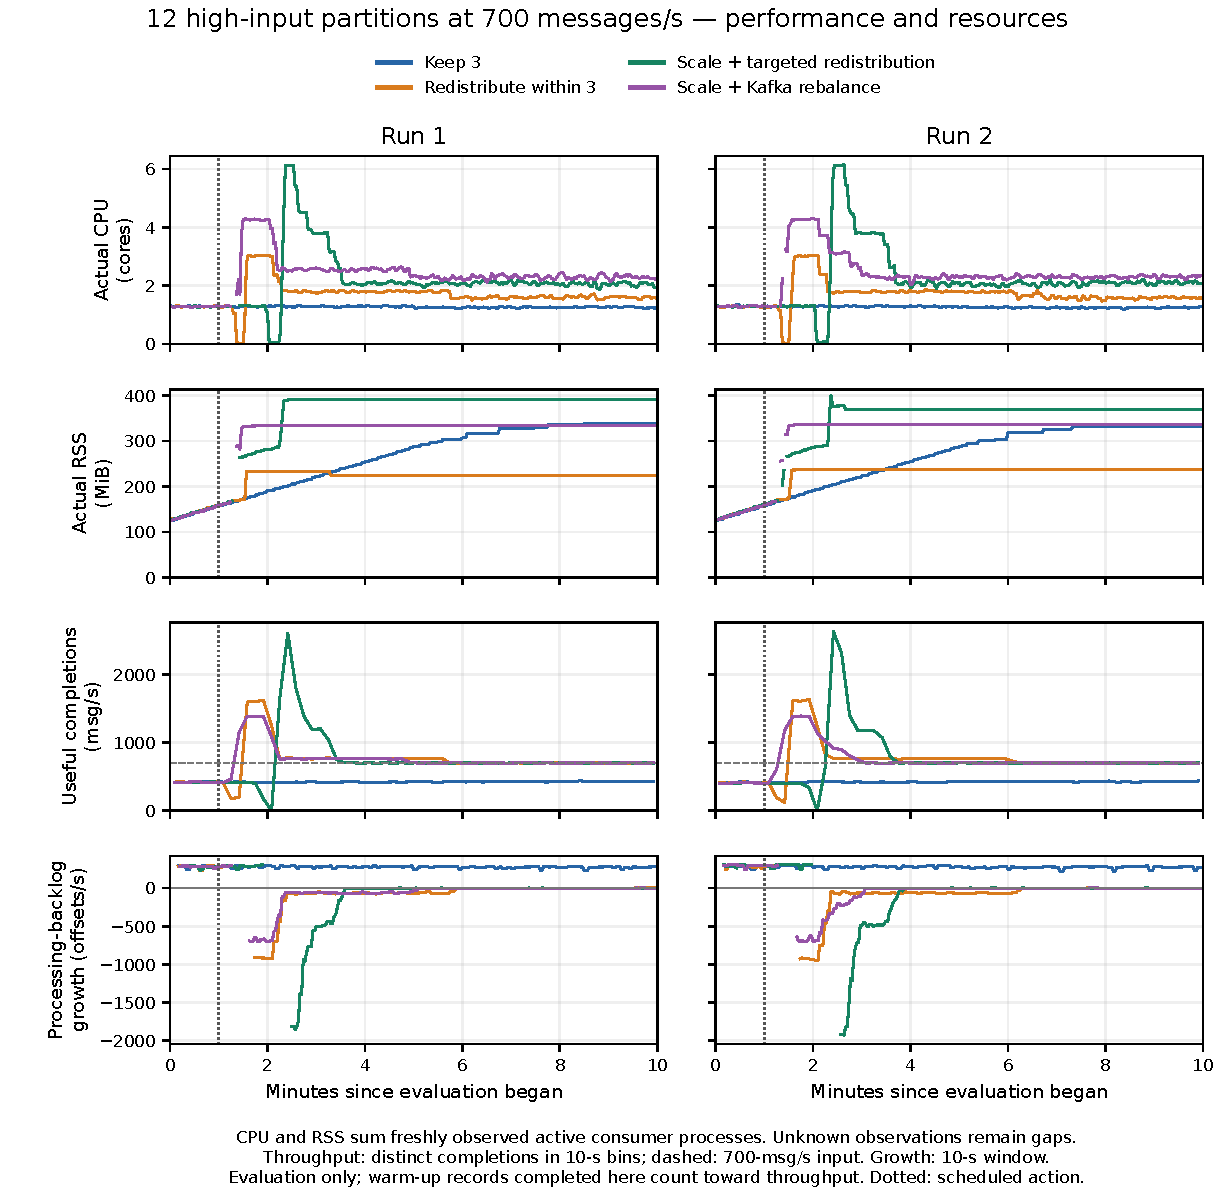
\includegraphics[width=\linewidth,height=.79\textheight,keepaspectratio]{figures/twelve-partition-compact-performance.pdf}
\caption{Actual consumer CPU and resident memory, useful completion throughput, and ten-second processing-backlog growth. Resource traces sum fresh measurements for all started consumer processes; an unavailable component leaves a gap. Requested resources and their integrals remain separate in the resource table.}
\label{fig:twelve-partition-compact-performance}
\end{figure}
\clearpage
\begin{figure}[p]
\centering
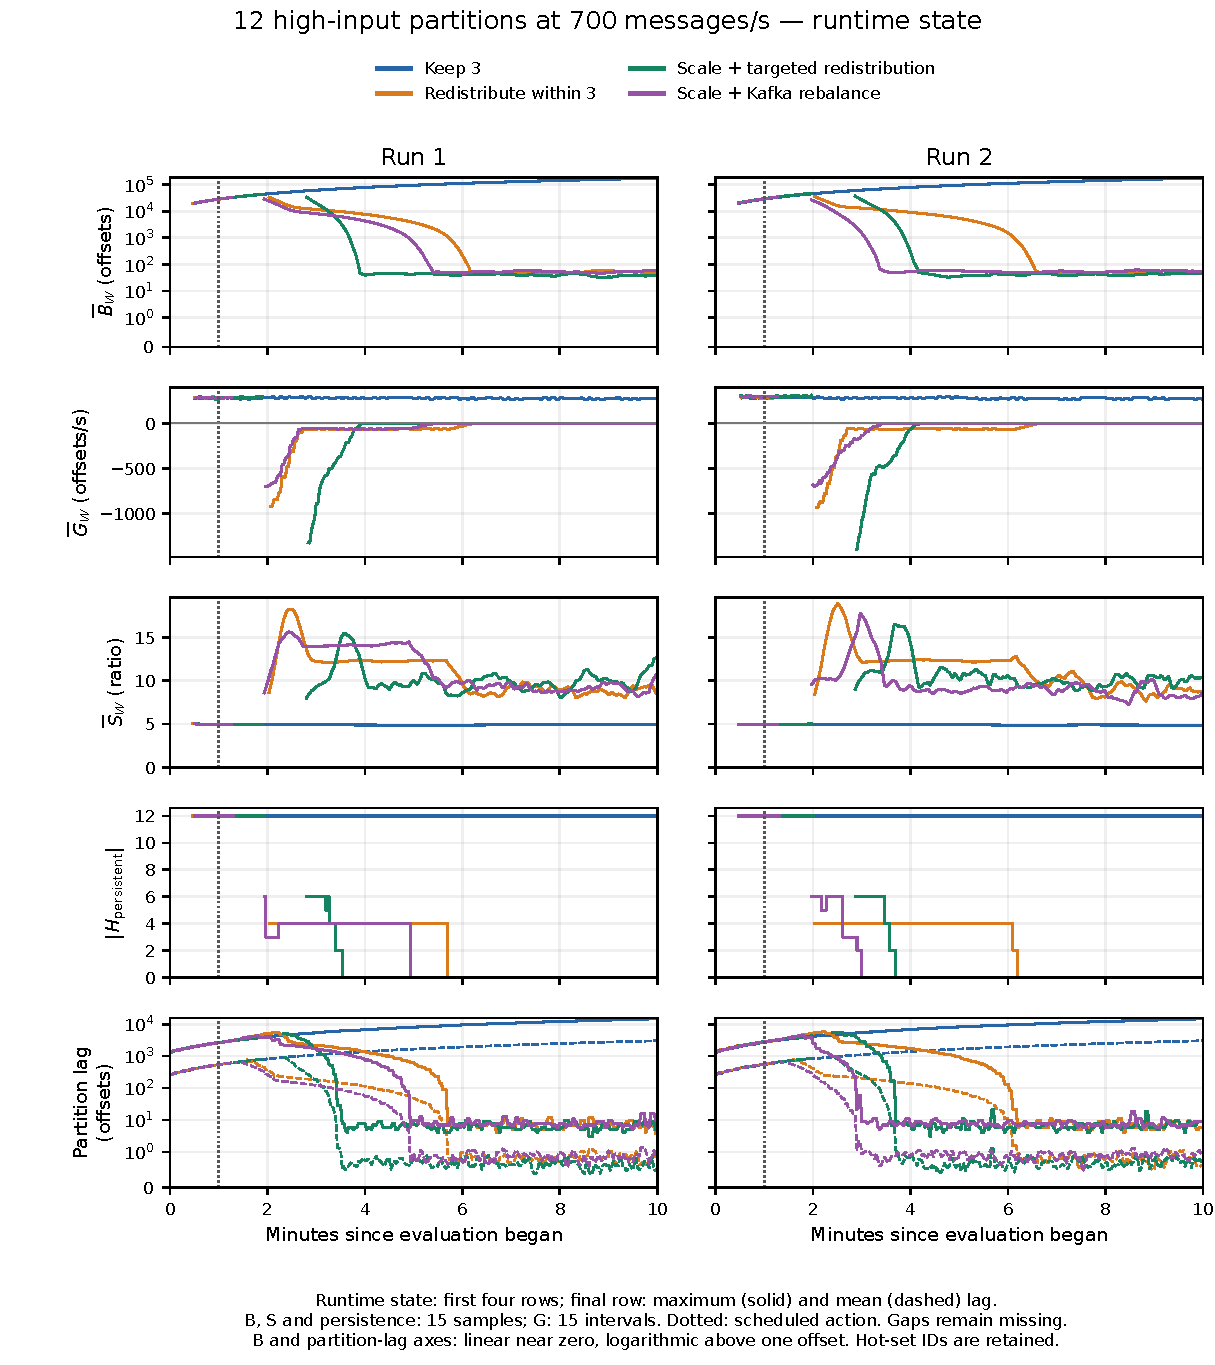
\includegraphics[width=\linewidth,height=.79\textheight,keepaspectratio]{figures/twelve-partition-runtime-state.pdf}
\caption{Reconstructed runtime state and partition-lag diagnostics. The first four rows show window-mean total lag, window growth, window-mean skew and persistent-hot count. The final row shows maximum and mean partition lag. Exact persistent-hot identifiers remain in the supporting data; the count alone does not identify a reassignment target. No scheduled action was selected by this reconstructed state.}
\label{fig:twelve-partition-runtime-state}
\end{figure}
\clearpage
